%!TEX TS-program = xelatex

% HSE Beamer Theme
% by Danil Fedorovykh
% http://hse.ru/staff/df
%
% Version 2.0 (English)
% January 2022

%%% Set up the free HSE Sans font
%%% https://www.hse.ru/info/brandbook/#font

\documentclass[aspectratio=169]{beamer}

\newbool{russian}
\booltrue{russian} % Uncomment if in Russian
\usepackage{HSE-theme/beamerthemeHSE} % Load HSE theme
\usepackage[no-math]{fontspec}      % fonts loading
\usepackage{caption}
\usepackage{subfigure}
\usepackage{subcaption}
\usepackage{hyperref}
\usepackage[dvipsnames]{xcolor}
\usepackage{ragged2e}
\captionsetup[figure]{labelformat=empty}
\captionsetup[subfigure]{labelformat=empty}
\renewcommand*{\thesubfigure}{(\arabic{subfigure})}
\setsansfont{HSE Sans}
%\graphicspath{{./images/}}
\graphicspath{{/home/llyy/Yandex.Disk/personal/knowledge/general/algorithms_course/repo/algorithms_course/5_simple_data_structures/lection/images}}


%%% Информация об авторе и выступлении
\title[Title]{Алгоритмы и структуры данных} 
\subtitle{Лекция 5. Простые структуры данных}
\author[Author's name]{Илья Сергеевич Бычков\\ \smallskip \scriptsize \url{ibychkov@hse.ru}}
\institute{НИУ ВШЭ - Нижний Новгород}
\date{\today}


\begin{document}

\frame[plain]{\titlepage}

%%%%%%%%%%%%%%%%%%%%%%%%%%%%%%%%%%%%%%%%%%%%%%%%%%%%%%%%%%%%%%%%%%%%%%%%%%%%%%%%%%%%%%%%%%%%%%%%%%
\begin{frame}[c]
%\frametitle{A first slide}

\begin{center}
\Huge Лекция 5.

\Huge Простые структуры данных
\end{center}

\end{frame}

%%%%%%%%%%%%%%%%%%%%%%%%%%%%%%%%%%%%%%%%%%%%%%%%%%%%%%%%%%%%%%%%%%%%%%%%%%%%%%%%%%%%%%%%%%%%%%%%%%
\begin{frame}
\frametitle{Алгоритмы поиска}
\framesubtitle{План лекции}

\begin{enumerate}
  \setcounter{enumi}{-1}
  \item{План лекции}
  \item{\textcolor{blue}{Связный список (linked list)}}
  \item{Стек (stack)}
  \item{Очередь (queue)}
\end{enumerate}
\end{frame}



%%%%%%%%%%%%%%%%%%%%%%%%%%%%%%%%%%%%%%%%%%%%%%%%%%%%%%%%%%%%%%%%%%%%%%%%%%%%%%%%%%%%%%%%%%%%%%%%%%
\begin{frame}
\frametitle{Связный список}
\framesubtitle{Связный список}
\justifying
\textcolor{red}{Связный список (linked list)} - это структура данных, состоящая  объектов специального вида, которые называются  \textcolor{blue}{узлами (nodes)}. Узлы хранят сами данные и связаны друг с другом с помощью указателей.\newline\newline
Каждый узел содержит одно или несколько полей для хранения данных\newline\newline
Каждый узел содержит указатель на следующий/предыдущий узел\newline\newline
Требуются указатели на первый/последний элементы списка\newline\newline
\end{frame}

%%%%%%%%%%%%%%%%%%%%%%%%%%%%%%%%%%%%%%%%%%%%%%%%%%%%%%%%%%%%%%%%%%%%%%%%%%%%%%%%%%%%%%%%%%%%%%%%%%
\begin{frame}
\frametitle{Связный список}
\framesubtitle{Структура node}
\justifying
\textcolor{red}{Связный список (linked list)}\newline

\begin{figure}
    \captionsetup[subfigure]{labelformat=empty}
    \centering
    \subfigure[{ \scriptsize Структура данных node, Источник - \href{https://www.learn-c.org/en/Linked_lists}{Ссылка}}]{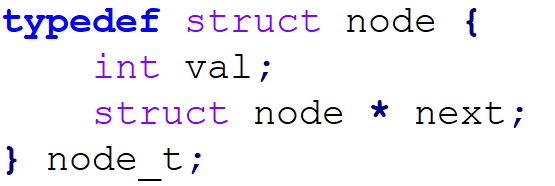
\includegraphics[width=60mm, height=22mm]{ll_node_code}} \quad\quad\quad
        \subfigure[{ \scriptsize Создание node, Источник - \href{https://www.learn-c.org/en/Linked_lists}{Ссылка}}]{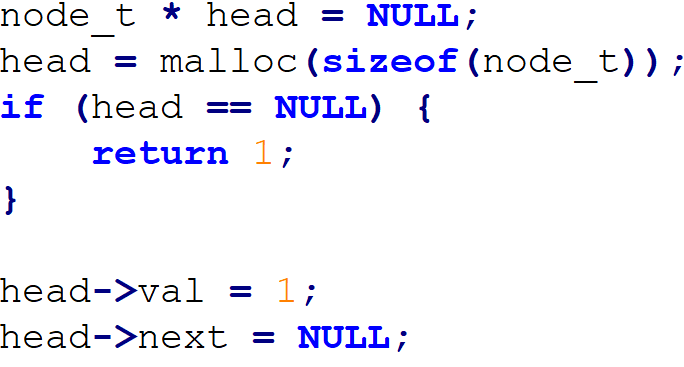
\includegraphics[width=65mm, height=40mm]{ll_node_create}} 
\end{figure}
\end{frame}

%%%%%%%%%%%%%%%%%%%%%%%%%%%%%%%%%%%%%%%%%%%%%%%%%%%%%%%%%%%%%%%%%%%%%%%%%%%%%%%%%%%%%%%%%%%%%%%%%%
\begin{frame}
\frametitle{Связный список}
\framesubtitle{Операции}
Основные операции\newline\newline
\textcolor{blue}{Вставка и удаление}
\begin{itemize}
  \item{В начало/конец списка}
  \item{До/после определенного значения}
  \item{До/после определенного адреса}
\end{itemize}
\textcolor{blue}{Поиск}
\begin{itemize}
  \item{По значению}
  \item{По позиции}
\end{itemize}
\begin{figure}
    \captionsetup[subfigure]{labelformat=empty}
    \centering
        \subfigure[{ \scriptsize Связный список, Источник - \href{https://www.geeksforgeeks.org/what-is-linked-list/}{Geeks4Geeks}}]{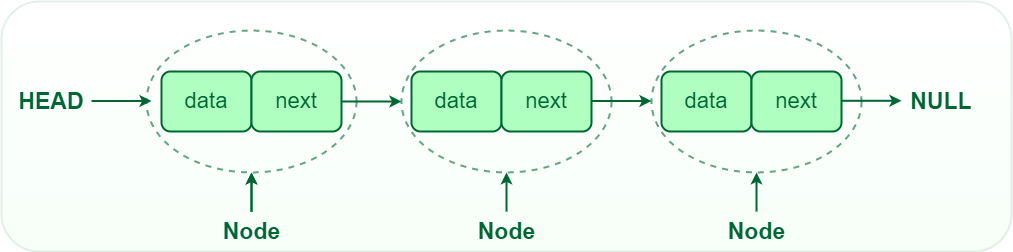
\includegraphics[width=80mm, height=20mm]{ll_single}} 
\end{figure}
\end{frame}

%%%%%%%%%%%%%%%%%%%%%%%%%%%%%%%%%%%%%%%%%%%%%%%%%%%%%%%%%%%%%%%%%%%%%%%%%%%%%%%%%%%%%%%%%%%%%%%%%%
\begin{frame}
\frametitle{Связный список}
\framesubtitle{Перебор связного списка}
\justifying
Перебор элементов связного списка

\begin{figure}
    \captionsetup[subfigure]{labelformat=empty}
    \centering
    \subfigure[{ \scriptsize Перебор элементов связного списка, Источник - \href{https://www.learn-c.org/en/Linked_lists}{Ссылка}}]{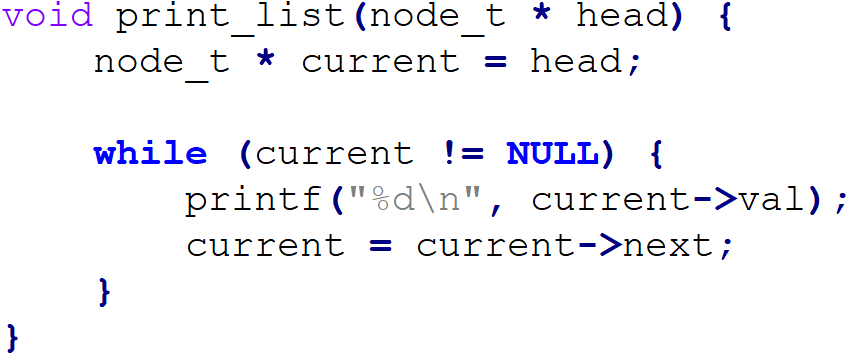
\includegraphics[width=90mm, height=40mm]{ll_traverse}}
\end{figure}
\end{frame}

%%%%%%%%%%%%%%%%%%%%%%%%%%%%%%%%%%%%%%%%%%%%%%%%%%%%%%%%%%%%%%%%%%%%%%%%%%%%%%%%%%%%%%%%%%%%%%%%%%
\begin{frame}
\frametitle{Связный список}
\framesubtitle{Вариации связных списков}
\justifying
\textcolor{red}{Односвязный список (singly linked list)} - состоит из узлов, которые хранят полезные данные и указатель на следующий

\begin{figure}
    \captionsetup[subfigure]{labelformat=empty}
    \centering
    \subfigure[{ \scriptsize Односвязный список, Источник - \href{https://www.sanfoundry.com/c-program-implement-singly-linked-list/}{Ссылка}}]{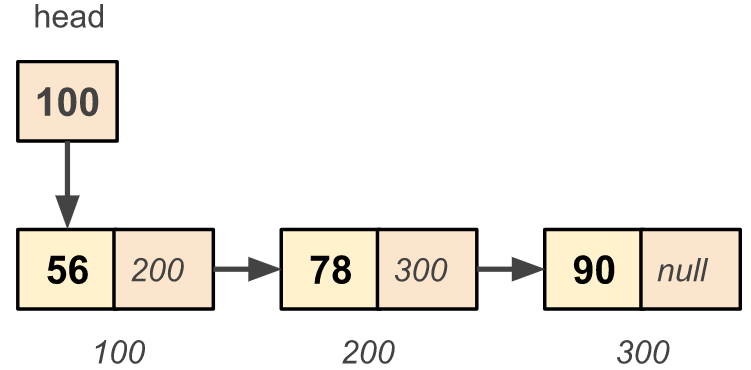
\includegraphics[width=90mm, height=40mm]{ll_single_variant}}
\end{figure}
\end{frame}

%%%%%%%%%%%%%%%%%%%%%%%%%%%%%%%%%%%%%%%%%%%%%%%%%%%%%%%%%%%%%%%%%%%%%%%%%%%%%%%%%%%%%%%%%%%%%%%%%%
\begin{frame}
\frametitle{Связный список}
\framesubtitle{Вариации связных списков}
\justifying
\textcolor{red}{Двусвязный список (doubly linked list)} - состоит из узлов, которые хранят полезные данные, указатели на предыдущий узел и следующий узел

\begin{figure}
    \captionsetup[subfigure]{labelformat=empty}
    \centering
    \subfigure[{ \scriptsize Двусвязный список, Источник - \href{https://www.geeksforgeeks.org/why-use-a-doubly-linked-list/}{Geeks4Geeks}}]{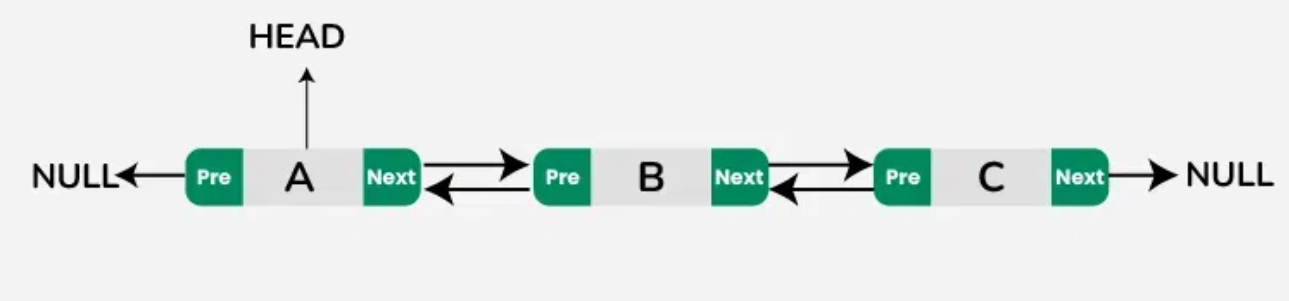
\includegraphics[width=130mm, height=40mm]{ll_doubly_variant}}
\end{figure}
\end{frame}

%%%%%%%%%%%%%%%%%%%%%%%%%%%%%%%%%%%%%%%%%%%%%%%%%%%%%%%%%%%%%%%%%%%%%%%%%%%%%%%%%%%%%%%%%%%%%%%%%%
\begin{frame}
\frametitle{Связный список}
\framesubtitle{Вариации связных списков}
\justifying
\textcolor{red}{Кольцевой связный список (circular linked list)} - разновидность связного списка, при которой первый элемент указывает на последний, а последний — на первый
\begin{figure}
    \captionsetup[subfigure]{labelformat=empty}
    \centering
    \subfigure[{ \scriptsize Односвязный список, Источник - \href{https://www.sanfoundry.com/c-program-implement-singly-linked-list/}{Ссылка}}]{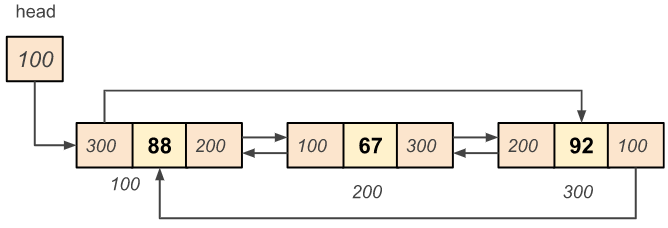
\includegraphics[width=120mm, height=40mm]{ll_circular_variant}}
\end{figure}
\end{frame}

%%%%%%%%%%%%%%%%%%%%%%%%%%%%%%%%%%%%%%%%%%%%%%%%%%%%%%%%%%%%%%%%%%%%%%%%%%%%%%%%%%%%%%%%%%%%%%%%%%
\begin{frame}
\frametitle{Связный список}
\framesubtitle{Сложность операций}
\justifying
\textcolor{red}{Односвязный список (singly linked list)}
\begin{figure}
    \captionsetup[subfigure]{labelformat=empty}
    \centering
    \subfigure[{ \scriptsize Односвязный список - сложность, Источник - Этот курс}]{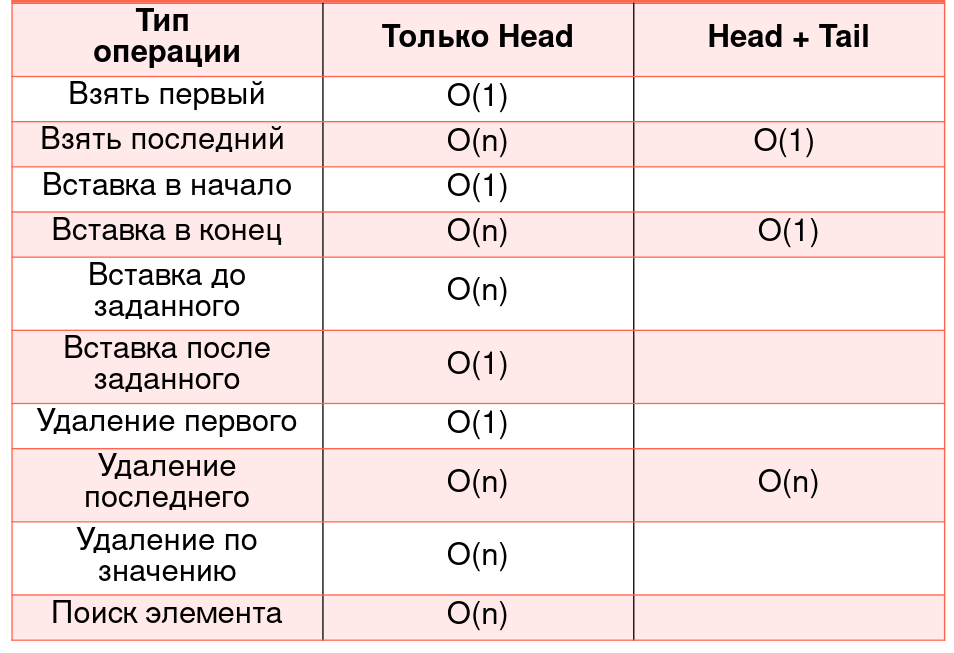
\includegraphics[width=85mm, height=55mm]{ll_singly_complexity_table}}
\end{figure}
\end{frame}

%%%%%%%%%%%%%%%%%%%%%%%%%%%%%%%%%%%%%%%%%%%%%%%%%%%%%%%%%%%%%%%%%%%%%%%%%%%%%%%%%%%%%%%%%%%%%%%%%%
\begin{frame}
\frametitle{Связный список}
\framesubtitle{Сложность операций}
\justifying
\textcolor{red}{Двусвязный список (doubly linked list)}
\begin{figure}
    \captionsetup[subfigure]{labelformat=empty}
    \centering
    \subfigure[{ \scriptsize Двусвязный список - сложность, Источник - Этот курс}]{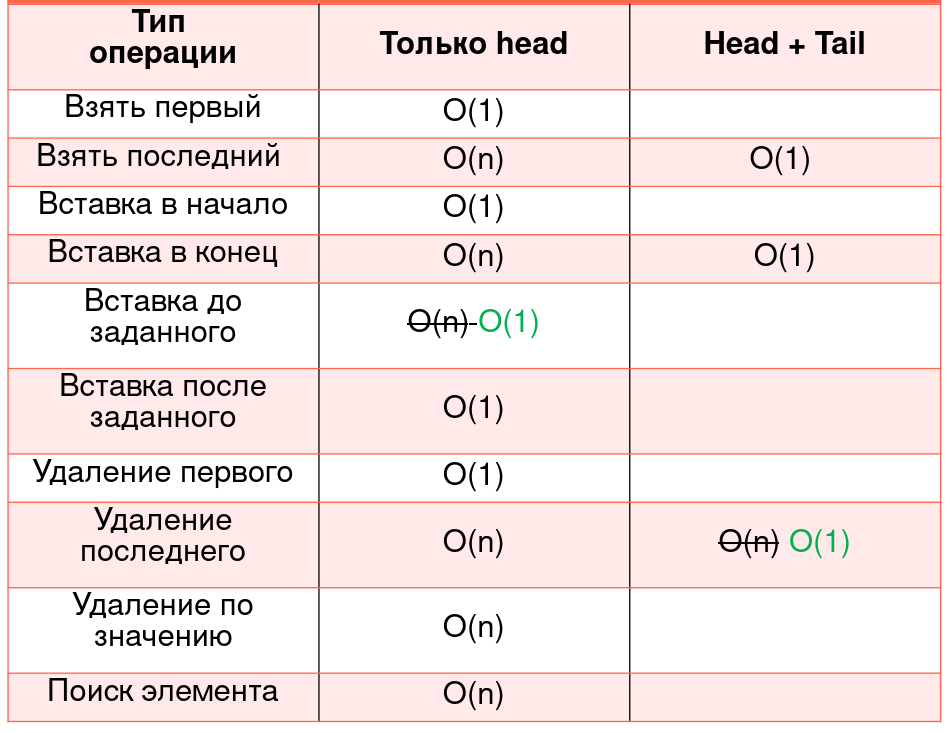
\includegraphics[width=80mm, height=55mm]{ll_doubly_complexity_table}}
\end{figure}
\end{frame}

%%%%%%%%%%%%%%%%%%%%%%%%%%%%%%%%%%%%%%%%%%%%%%%%%%%%%%%%%%%%%%%%%%%%%%%%%%%%%%%%%%%%%%%%%%%%%%%%%%
\begin{frame}
\frametitle{Связный список}
\framesubtitle{Преимущества и недостатки}
\justifying
Связные списки - Преимущества и недостатки
\begin{figure}
    \captionsetup[subfigure]{labelformat=empty}
    \centering
    \subfigure[{ \scriptsize Связные списки - Преимущества и недостатки, Источник - Этот курс}]{
\includegraphics[width=135mm, height=50mm]{ll_pros_cons}}
\end{figure}
\end{frame}

\end{document}